%iffalse
\let\negmedspace\undefined
\let\negthickspace\undefined
\documentclass[journal,12pt,onecolumn]{IEEEtran}
\usepackage{cite}
\usepackage{amsmath,amssymb,amsfonts,amsthm}
\usepackage{algorithmic}
\usepackage{graphicx}
\usepackage{textcomp}
\usepackage{xcolor}
\usepackage{txfonts}
\usepackage{listings}
\usepackage{enumitem}
\usepackage{mathtools}
\usepackage{gensymb}
\usepackage{comment}
\usepackage[breaklinks=true]{hyperref}
\usepackage{tkz-euclide} 
\usepackage{listings}
\usepackage{gvv}                                        
\def\inputGnumericTable{}                                 
\usepackage[latin1]{inputenc}                                
\usepackage{color}                                            
\usepackage{array}                                             
\usepackage{longtable}                                       
\usepackage{calc}                                             
\usepackage{multirow}                                         
\usepackage{hhline}                                           
\usepackage{ifthen}                                           
\usepackage{lscape}
\usepackage{multicol}

\newtheorem{theorem}{Theorem}[section]
\newtheorem{problem}{Problem}
\newtheorem{proposition}{Proposition}[section]
\newtheorem{lemma}{Lemma}[section]
\newtheorem{corollary}[theorem]{Corollary}
\newtheorem{example}{Example}[section]
\newtheorem{definition}[problem]{Definition}
\newcommand{\BEQA}{\begin{eqnarray}}
\newcommand{\EEQA}{\end{eqnarray}}
\newcommand{\define}{\stackrel{\triangle}{=}}
\theoremstyle{remark}
\newtheorem{rem}{Remark}
\begin{document}

\bibliographystyle{IEEEtran}
\vspace{3cm}

\title{NCERT - 9.4.15}
\author{EE224BTECH11044 - Muthyala koushik
}
\maketitle
\bigskip

\renewcommand{\thefigure}{\theenumi}
\renewcommand{\thetable}{\theenumi}
\textbf{\section{DIFFERENTIAL EQUATIONS}}

\textbf{Question:} $2xy+y^2-2x^2 \frac{dx}{dy}=0$; $y=2$ when $x=1$ \\ 

\solution\textbf{(Theoretical Solution)} The given differential equation can be written as

\begin{align}
    \frac{dy}{dx} = \frac{y}{x} + \frac{y^2}{2x^2}
\end{align}

To solve it, we make the substitution

\begin{align}
    y = xt
\end{align}

Differentiating equation $(2)$ with respect to $x$, we get

\begin{align}
    \frac{dy}{dx} = t + x\frac{dt}{dx}
\end{align}

Substituting the value of $y$ and $\frac{dy}{dx}$ in equation $(1)$, we get

\begin{align}
    t + \frac{t^2}{2} &= t + x\frac{dt}{dx} \\
    \frac{t^2}{2} &= x\frac{dt}{dx} \\
    \frac{dx}{2x} &= \frac{dt}{t^2} \\
    \int \frac{dx}{2x} &= \int \frac{dt}{t^2} \\
    \frac{\ln{x}}{2} &= -\frac{1}{t} + c
\end{align}

Replacing $t$, we have

\begin{align}
    \frac{\ln{x}}{2} &= -\frac{x}{y} + c
\end{align}

Substituting $x = 1$, $y = 2$ to find $c$, we get

\begin{align}
    \frac{\ln{1}}{2} &= -\frac{1}{2} + c \\
    c &= \frac{1}{2}
\end{align}

By solving, we obtain $y$ as

\begin{align}
    y &= \frac{2x}{1 - \ln{x}}
\end{align}

\textbf{Solution by the method of finite differences:}\\
\begin{align}
    \frac{dy}{dx} = \frac{y}{x} + \frac{y^2}{2x^2}
\end{align}

Using the method of finite differences, we approximate the derivative as
\begin{align}
    \frac{dy}{dx} \approx \frac{y_{n+1} - y_n}{h}
\end{align}
 
Substitute equation$(14)$ in equation$(13)$
\begin{align}
	\frac{y_{n+1} - y_n}{h} &=  \frac{y_n}{x_n} + \frac{{y_n}^2}{2{x_n}^2}\\
	y_{n+1}-y_n &= h  (\frac{y_n}{x_n} + \frac{{y_n}^2}{2{x_n}^2})\\
	y_{n+1} &= y_n+h(\frac{y_n}{x_n} + \frac{{y_n}^2}{2{x_n}^2})
\end{align}

The initial conditions are given as:  $x_0 = 1$, $y_0 = 2$, $h=0.005$. Using the recurrence relation $(17)$, we compute values of $x_n$ and $y_n$. These values can be used to approximate the solution numerically for a given range of $x$.

\begin{figure}[h]
	\centering
	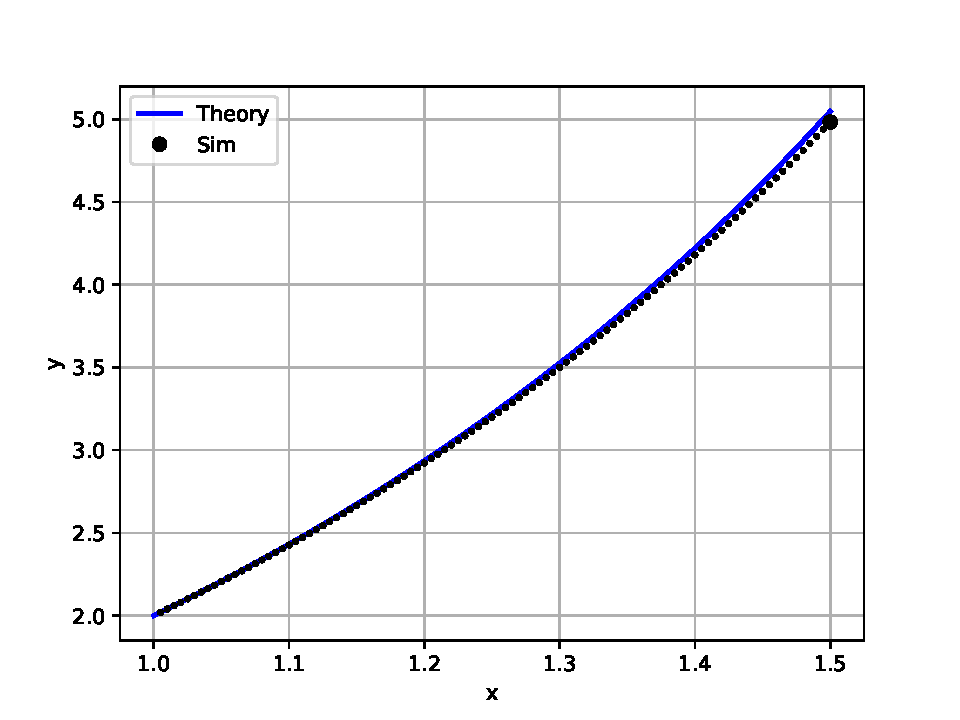
\includegraphics[width=\columnwidth]{figs/fig.pdf}
	\caption{Solution of given DE}
	\label{fig}
\end{figure}

\end{document}
